%!TEX root = project.tex

\chapter*{About this project}

\paragraph{Abstract}


\paragraph{Authors}


\chapter*{Acknowledgements}


\chapter{Introduction}
\par Par

\par Test Par end reference\cite{NameOfreff}.

\chapter{Context}

\section{Objectives}
The overall objective of our project:

\begin{enumerate}
    \item \textbf{Objective1} About objective:
    \begin{itemize}
        \item Database 
        \item Authentication 
    \end{itemize}
    \item \textbf{Objective 2} The description and so on.
\end{enumerate}

\section{Project Links}
Links to this document.

\paragraph{Links}
\begin{itemize}
\item https://github.com
\item https://github.com
/
\end{itemize}

\section{Chapters Review}
Description of chapters

\subsection{Methodology}
Description of chapters

\subsection{Technology Review}
Description of chapters

\subsection{System Design}
Description of chapters

\subsection{System Evaluation}
Description of chapters

\subsection{Conclusion}
Description of chapters

\chapter{Methodology}
Description of chapters

\section{Agile Development}
aaaaaaaaaaaaaaaaaaaaaaaaaaaaaaaaa\par
blabla\cite{FirstnameLastname}.\par
bbbbbbbbbbbbbbbbbbbbbbbbbbbbbbbbbb\cite{NameOfreff}.

\section{Testing}
tttttttttttttttttttttttttttttt
\cite{FirstnameLastname}.


\chapter{Technology Review}
tehhhhhhhhhhhhhhhhhhhhhhhhhhhhhhh

\section{Development Environment}
different programming tools


\subsection{GitHub}

Some sample git commands used are as follows:
\begin{itemize}

    \item git add .\par
    Add folders or files to be tracked by github so later they can be
    committed and pushed on to github account.

\end{itemize}


A sample JUnit test case can be found below\cite{JUnit}:

\begin{minted}{java}

public class MyTests {

\end{minted}

\subsection{Ionic}

\subsection{MongoDB}
\cite{mLab}.\\
\\
A sample of the MongoDB stucture is as follows\cite{WilliamZola}:
\begin{minted}{json}
{
    "_id" : 1

\end{minted}

\section{Bootstrap}

\section{JQuery}


\section{JavaScript}

\begin{minted}{js}
// Function is called, return value will end up in x
var x = myFunction(4, 3);   
}
\end{minted}

\section{CSS}


\begin{minted}{css}
body {
    background-color: lightblue;
}
\end{minted}

\chapter{System Design}

\begin{figure}[h]
\centering
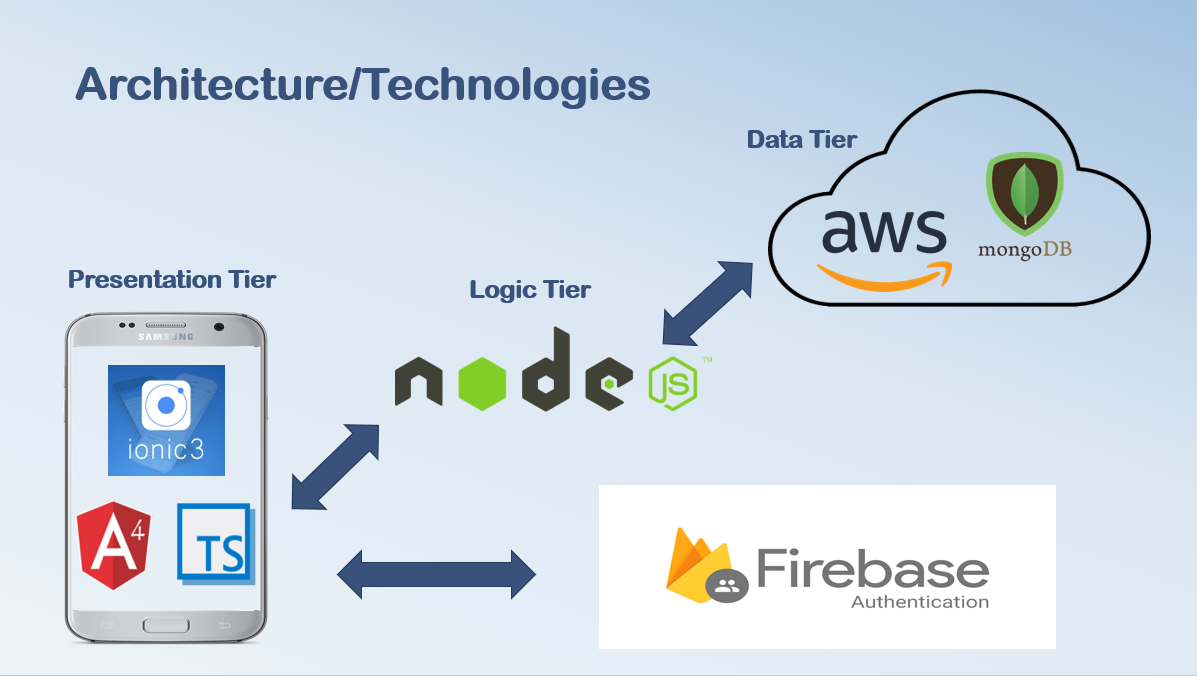
\includegraphics[width=14cm, height=7cm]{img/Architecture}
\caption{System Architecture.}
\end{figure}

\section{System Backend}

\subsection{Databases}
We chose databases..


\subsection{Security}

\section{Front End }

\subsection{Login/Register}
\par The login 

\begin{figure}[h]
\centering
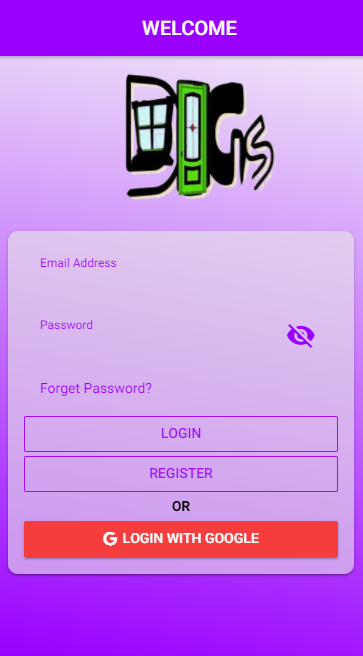
\includegraphics[width=8cm, height=16cm]{img/loginScreen}
\caption{Login Page}
\end{figure}

\subsection{Room page...}


\chapter{System Evaluation}
This Chapter evaluate the application
\begin{itemize}
    \item Scalability
    \item Robustness
    \item Maintainability
    \item Extensibility
\end{itemize}

\par \textbf{Scalability:} 

\par \textbf{Robustness:}.

\par \textbf{Maintainability:}

\par \textbf{Extensibility:} T

\section{Testing}

\section{Outcomes VS. Objectives}

\section{Limitations}

\section{Opportunities}

\chapter{Conclusion}


\begin{itemize}
\item A Test

\item A Test2
\item A Test3
\end{itemize}
A Test4
\section{Future Development}

\chapter{Appendix}

\textbf{Project Source Code Link: }link to github \\
\textbf{Project Documentation Link: }https://github.com/Chrissweir/Final-Year-Project/blob/master/project.pdf \\

